% !TEX root=../../Thesis.tex
\chapter{Accounting for the uncertainty}\label{ch:uncertainty}
% \begin{center}
% 	\textit{\textbf{RQ 2: In what way can an \gls{rl} agent utilize the uncertainty of its predictions and actions?}}
% 	% \textit{\textbf{RQ 4: How can the quality of a RL agent be improved by accounting for uncertainty?}}
% 	\end{center}
% 	\vspace{12pt}

The previous chapter formulated the \gls{pomdp} and introduced how deep Q-learning methods can be utilized to create decision-making agents capable of navigating intersections. A significant advantage of RL methods is their scalability to different scenarios through appropriate training. However, a drawback of deep Q-learning methods, is the use of neural networks, which provide a black-box solution without indicating any confidence or uncertainty in their decisions.

This chapter presents two approaches to estimating the uncertainty: \paperEnsamble \ addresses the uncertainty in the output of the \gls{dqn}, and \paperBelief \ addresses the uncertainty in the intention estimation that is fed as an input to the \gls{dqn}.
To demonstrate the effect of accounting for uncertainty, the results include two types of experiments. In the first type, the trained agent is evaluated on scenarios within the training set. In the second type, the agent is evaluated on scenarios outside the training set. Both types of experiments are conducted using the same simulation environment described in Section~\ref{ch:simulation_env}.

\section{Estimating the uncertainty of the Q-value}
\label{ch:ensamble}
To estimate the uncertainty in the $Q$-value of the trained agent, \paperEnsamble \ employed statistical bootstrapping to train an ensemble of neural networks on different subsets of the available experience. This ensemble provides a distribution over the estimated $Q$-values for any input. A better Bayesian posterior is obtained by adding different \gls{rpf} to each ensemble member~\cite{Osband2018}.
The $Q$-values of each ensemble member $k$ is then calculated as the sum of two neural networks, $f$ and $p$, with the same architecture, i.e.,
%
\begin{align}
	Q_k(s,a) = f(s,a;\theta_k) + \beta p(s,a;\hat{\theta}_k).
\end{align}
Here, the weights $\theta_k$ of network $f$ are trainable, and the weights $\hat{\theta}_k$ of the prior network $p$ are fixed to the randomly initialized values. A parameter $\beta$ scales the importance of the networks. With the two networks, the loss function in Eq.~\ref{eq:lossDQN} becomes
%
\begin{align}
	\label{eq:loss_boot}
	L(\theta_k) = \mathbb{E}_M \Big[ & (r + \gamma \max_{a'} (f_{\theta^-_k}+\beta p_{\hat{\theta}_k})(s',a') \nonumber \\
	& - (f_{\theta_k}+ \beta p_{\hat{\theta}_k})(s,a) )^2 \Big].
\end{align} 

% One limitation of the \gls{dqn} algorithm is that only the maximum likelihood estimate of the $Q$-values is returned. The risk of taking a particular action can be approximated as the variance in the estimated $Q$-value~\cite{Garcia2015}. 
% The basic idea is to train an ensemble of neural network on different subsets of the available experience. The ensemble will then provide a distribution of $Q$-values, which can be used to estimate the variance. Osband et al. extended the ensemble method by adding a \gls{rpf} to each ensemble member, which gives a better Bayesian posterior~\cite{Osband2018}. The $Q$-values of each ensemble member $k$ is then calculated as the sum of two neural networks, $f$ and $p$, with equal architecture, i.e.,
%

The training process of an ensamble \gls{rpf} is described by Algorithm~\ref{alg:ensamble_training}. 
An ensemble of $K$ \gls{dqn} are first initialized randomly. Each ensemble member is also assigned a separate experience replay memory buffer $m_k$. 
For each new episode, a random ensemble member $\nu$ is selected and used to take greedy actions throughout the episode, which corresponds to an approximate Thompson sampling approach to the exploration vs.~exploration dilemma.
Each new experience $e = (s_i, a_i, r_i, s_{i+1})$ is then added to the separate replay buffers $m_k$ with probability $p_\mathrm{add}$. The trainable weights of each ensemble member are then updated by uniformly sample a mini-batch $M$ of experiences and using \gls{sgd}.

\begin{algorithm}[h]
	\caption{Ensemble RPF training process}\label{alg:ensamble_training}
	\begin{algorithmic}[1]
		\For{$k \gets 1$ to $K$}
			\State Initialize $\theta_k$ and $\hat{\theta}_k$ randomly
			\State $m_k \gets \{\}$
		\EndFor
		\State $i \gets 0$
		\While{networks not converged}
			\State $s_i \gets $ initial random state
			\State $\nu \sim \mathcal{U}\{1,K\}$%, where $k \in \mathbb{N}$
			\While{episode not finished}
				\State $a_i \gets \argmax_{a} Q_\nu(s_i,a)$
				\State $s_{i+1}, r_i \gets $ \Call{StepEnvironment}{$s_i, a_i$}
				% \For{$i \in \{1,\dotsc,K\}$}
				\For{$k \gets 1$ to $K$}
					\If{$p \sim \mathcal{U}(0,1) < p_\mathrm{add}$}%, where $p \in \mathbb{R}$ 
						\State $m_k \gets m_k \cup \{(s_i, a_i, r_i, s_{i+1})\}$
					\EndIf
					\State $M \gets $ sample mini-batch from $m_k$
					\State update $\theta_k$ with SGD and loss $L(\theta_k)$
				\EndFor
				\State $i \gets i + 1$
			\EndWhile
		\EndWhile
	\end{algorithmic}
\end{algorithm}

The agent's uncertainty in choosing different actions can be defined as the coefficient of variation $c_\mathrm{v}(s,a)$ of the $Q$-values of the ensemble members~\cite{Hoel2020}.
A threshold $c_\mathrm{v}(s,a)$ can then be used to determine whether an action has an acceptable level of uncertainty.

A high uncertainty, where $c_\mathrm{v}(s,a) > c_\mathrm{v}^\mathrm{safe}$, indicates that $(s,a)$ is outside the training distribution. 
When the agent is fully trained, the policy $\pi$ chooses actions by maximizing the mean of the $Q$-values of the ensemble members, with the restriction $c_\mathrm{v}(s,a) < c_\mathrm{v}^\mathrm{safe}$, i.e.,
%
\begin{equation}
	\begin{aligned}
		\pi = \argmax_{a} \frac{1}{K} \sum_{k=1}^K Q_k(s,a),\\
		\textrm{s.t.} \quad c_\mathrm{v}(s,a) < c_\mathrm{v}^\mathrm{safe}.
	\end{aligned}
\end{equation}

If no action within the action space satisfies the restriction, a predefined backup action $a_\mathrm{safe}$ is chosen instead. This $a_\mathrm{safe}$ can be something like a collision avoidance measure, such as emergency braking.
%
% In a situation where no possible action fulfills the confidence criterion, a fallback action $a_\mathrm{safe}$ is chosen.

%  In this thesis, the benefit of this estimate is demonstrated by applying a backup policy $\pi_\mathrm{backup}(s)$ if an action has an unacceptable level of uncertainty, i.e., the trained agent follows the policy
% %
% \begin{align}
%     \pi_{\sigma_\mathrm{e}}(s) = 
%     &\begin{cases} \argmax_{a} \mathbb{E}_k[Q_k(s,a)], & \mathrm{if\ } \mathrm{Var}_k[Q_k(s,a)] < \sigma^2_\mathrm{e}, \\
%     \pi_\mathrm{backup}(s), & \mathrm{otherwise}.
%     \end{cases}
% \end{align}

\subsection{Results for scenarios within the training set}

This section shows the results of the ensemble \gls{rpf} method compared to the \gls{dqn} method used in \paperLSTM, but without the \gls{lstm} layer.
The ensemble \gls{rpf} method outperforms the \gls{dqn} method when the agents are tested on scenarios that are similar to the training scenarios. When the fully trained ensemble \gls{rpf} agent is exposed to situations that are outside the training distribution, the agent indicates a high uncertainty and chooses safe actions, whereas the \gls{dqn} agent sometimes collides with other vehicles.

\begin{figure}[h]
	\mbox{\parbox{\textwidth}{
	\centering
	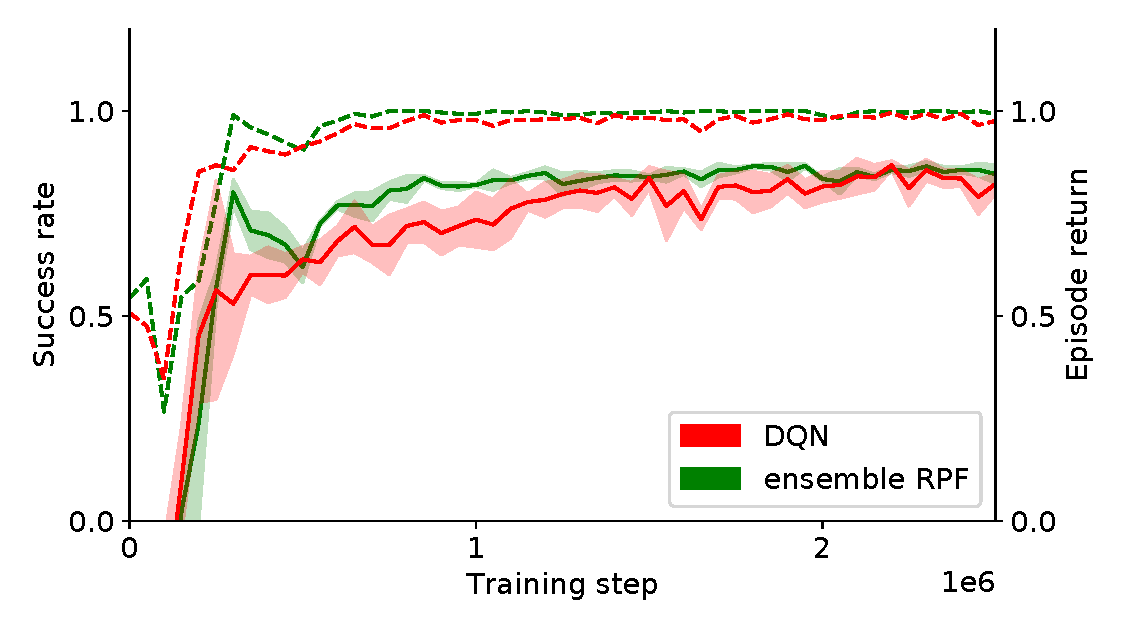
\includegraphics[width=0.7\columnwidth]{YourThesis/papers/ensamble/figures/return_success_rate_2_wo_type_3_fonts.pdf}
	}}
	\caption{Proportion of test episodes where the ego vehicle reached its goal (dashed), and episode return (solid), over training steps for the ensemble \gls{rpf} and \gls{dqn} methods. The shaded areas show the standard deviation for $5$ random seeds.}
	\label{fig:thesis_RPFreturnAndSuccess}
\end{figure}

The average return and the average proportion of episodes where the ego vehicle reached the goal, as a function of number of training steps, is shown in Figure~\ref{fig:thesis_RPFreturnAndSuccess}, for the test episodes. The figure also shows the standard deviation for $5$ random seeds, which generates different sets of initial parameters of the networks and different training episodes, whereas the test episodes are kept fixed. The results show that the ensemble RPF method both learns faster, yields a higher return, and causes less collisions than the \gls{dqn} method. %A few collisions still remain, but how they can be mitigated is shown below.
%

\begin{figure}[h]
	\mbox{\parbox{\textwidth}{
	\centering
		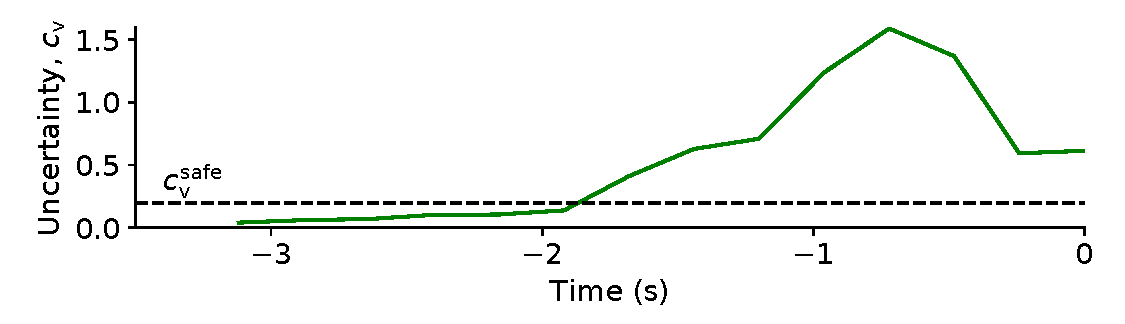
\includegraphics[width=0.8\columnwidth]{YourThesis/papers/ensamble/figures/uncertainty_at_collision_wo_type_3_fonts.pdf}
		}}
		\caption{Uncertainty $c_\mathrm{v}$ during the time steps before one of the collisions in the test episodes, within the training distribution. The collision occurs at $t=0$ s.}
	\label{fig:RPFcvDuringCrash}
\end{figure}

% As shown in Figure~\ref{fig:thesis_RPFreturnAndSuccess}, occasional collisions still occur during the test episodes when deploying the fully trained ensemble RPF agent. 
Upon analyzing the scenarios with collisions using the DQN agent, it was observed that in one particular example, the agent fails to brake sufficiently in zone 3 (from Figure~\ref{fig:zones}) and takes an incorrect action in zone 2, resulting in a collision in zone 1. 
In contrast, in the same scenario with the ensemble \gls{rpf} agent, Figure~\ref{fig:RPFcvDuringCrash} show that the estimated uncertainty increases significantly during the time before the collision (zone 2), when the incorrect actions was taken. 
By applying the confidence criterion, the agent, aware of high uncertainty, brakes early enough in zone 2, thus avoiding collisions. This confidence criterion was applied to all test episodes, effectively eliminating all collisions for scenarios within the training set.


\subsection{Results for scenarios outside the training set}
\begin{figure}[h]
	
	\mbox{\parbox{\textwidth}{
		\centering
	\begin{subfigure}[]{0.99\columnwidth}
	\centering
		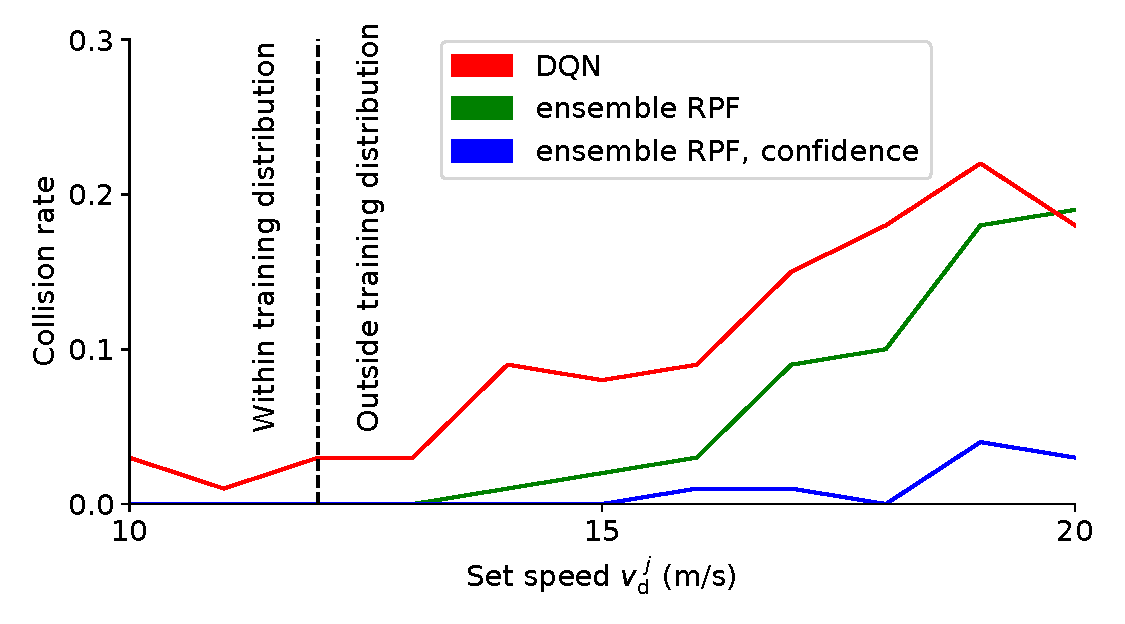
\includegraphics[width=0.7\columnwidth]{YourThesis/papers/ensamble/figures/collisions_outside_distribution_2_wo_type_3_fonts.pdf}
		\caption{Proportion of collisions.}
	\end{subfigure}
	
	\vspace{5pt}
	
	\begin{subfigure}[]{0.99\columnwidth}
	\centering
		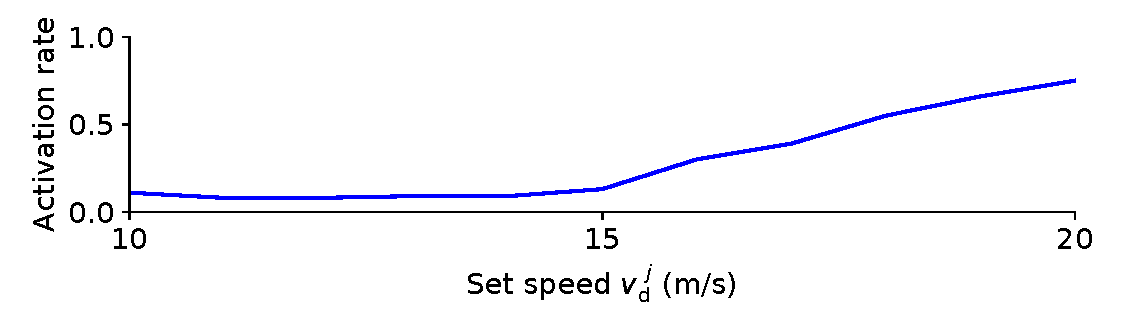
\includegraphics[width=0.7\columnwidth]{YourThesis/papers/ensamble/figures/activation_rate_2_wo_type_3_fonts.pdf}
		\caption{Proportion of episodes where $a_\mathrm{safe}$ was used at least once.}
	\end{subfigure}
	\caption{Performance of the ensemble RPF agent, with and without the confidence criterion, and the DQN agent, in test episodes with different velocities for the surrounding vehicles. 
	}
	\label{fig:RPFperformanceOutsideDistribution}
	}}
\end{figure}

To evaluate the agents' ability to detect unseen situations, a fully trained ensemble RPF agent was tested in scenarios outside the training distribution. The same testing scenarios as in the previous section were used, with the exception that the speed of the surrounding vehicles was set to a single deterministic value, which was varied during different runs in the range $v_n\in[10,20]$ m/s. 
The proportion of collisions as a function of set speed of the surrounding vehicles is shown in Figure~\ref{fig:RPFperformanceOutsideDistribution}, along with the proportion of episodes where the confidence criterion was violated at least once. The figure demonstrates that by accounting for the uncertainty of the $Q$-value and the use of the confidence criterion some collisions can be avoided.
% Additionally, violations of the criterion increase as the speed of the surrounding vehicles increases, indicating that the scenarios are moving further from the training distribution.


\section{Estimating the uncertainty of the input}
The ensemble RPF agent avoided collisions by not taking a bad action in zone 2, by accounting for the uncertainty of the Q-value estimate. However, can further reductions in collisions be achieved by accounting for uncertainty in the input? 
In \paperBelief, the uncertainty regarding the intention state $\zeta_n$ is managed using a belief state represented as a probability distribution over possible states. This distribution, referred to as intention distributions, is generated using a particle filter. Based on these distributions, two methods were proposed: QMDP-IE and QID.

% \begin{figure}[!h]
% 	\centering
% 			\begin{tikzpicture}
    %\node[](obs_eq) at (-2.5,2) {$o = (p^\mathrm{ego}_\mathrm{goal},p^\mathrm{ego}_\mathrm{int}, v^\mathrm{ego}, t_\mathrm{stop}, \{\hat{p}^{j}_\mathrm{int}, \hat{v}^j\}_{j=1}^N).$};
    %\node (ego_state) at (-0.7, 0.8) {$\hat{s}_e = (p^\mathrm{ego}_\mathrm{goal},p^\mathrm{ego}_\mathrm{int}, v^\mathrm{ego}, t_\mathrm{stop})$};

    % \node (target_state) at (-2.9, -7) {$\hat{s}_j = \{p^{j}_\mathrm{int}, v^j, i^j\}_{j=1}^N$};
    % \node (intent_state) at (-3, -7.5) {Intent from eq.$(20)$};

    %\node (target_state) at (-0.7, -2.5) {$\hat{s}_j = \{p^{j}_\mathrm{int}, v^j\}_{j=1}^N$};
    %\node (intent_state) at (-1, -5.2) {$\hat{i}^j (19)$};

    \def\pfx{-2.2}
    \def\pfy{-1.8}
    \def\radius{.95}

    % \node[](obs) at (\pfx,0) {$o$};
    \node[](ego_state) at (-0.5,0.3) {$s_\mathrm{ego}$};
    % \node[](target_state) at (0.1,-.8) {$\{\hat p_n, \hat v_n \}^N_{n=1}$};
    \node[](target_state) at (-.3,-.8) {$o_{1:N}$};
    \node[](target_observation) at (-1.7,-.8) {$o_{1:N}$};
    \node[](target_state) at (-.5,\pfy+.3) {$\zeta_{n}$};
    \node[](target_state) at (.5,\pfy+.3) {$s_{1:N}$};

        \node[](obs) at (\pfx-.9,0) {$o$};
    \node[circle, draw=black, minimum size=2.2] (split) at (\pfx, 0) {}; 
    % \node[](ego_state) at (.3,0.4) {$\{s_\mathrm{ego} \}_{m=1}^M$};
    % \node[](target_state) at (0.2,\pfy+.3) {$\{x_{m} \}_{m=1}^M$};
    % \node[](target_observation) at (-1,-.5) {$o_{1:N}$};
    
    \makepointcloud

    \def\BeliefSize{1}
    \def\BeliefDepth{1}
    % \baseinput{1};

    \node[draw,fill=blue!5,thick,inner sep=3pt,minimum width=1mm, minimum height=38mm, dashed, align=center] (dqn) at (2,\pfy/2-.3,0){DQN \\ Z=1 \\ See \\ Figure \ref{fig:network}};

    
    \pic[shift={(0.5,0,0)}] at (dqn.east) 
    {Box={
        name=q_particle,
        caption=,
        xlabel={{2, }},
        ylabel= ,
        zlabel=\BeliefSize,
        fill=\SoftmaxColor,
        opacity=0.8,
        height=4,
        width=1.5,
        depth=\BeliefDepth
        }
    };

    \pic[shift={(1.1,0,0)}] at (pf) 
    {Box={
        name=approx,
        caption=$ $,
        xlabel={{ , }},
        ylabel= ,
        zlabel= ,
        fill=\SoftmaxColor,
        opacity=0.8,
        height=4,
        width=1,
        depth=\BeliefDepth
        }
    };

    \draw [connection]  (dqn.east)  -- node {\midarrow} (q_particle-west);
    % \draw [connection]  (input_ego-east)  -- node {\midarrow} ($(input_ego-east)+(1.1,0)$);
    % \draw [connection]  (input_target1-southeast)  -- node {\midarrow} ($(input_target1-southeast)+(1.1,0)$);
    %\node (space) at (,0) {};		
    \draw [connection]  (split)  -- node {\midarrow} (pf);
    \draw [connection]  (obs)  -- node {\midarrow} (split);
    % \draw [connection]  (obs)  -- node {\midarrow} (input_ego-west);
    % \draw [connection]  (obs)  -- node {\midarrow} (input_target1-southwest);
    \draw [connection]  (split)  -- node {\midarrow} ($(split)+(3.35,0)$);
    \draw [connection]  (split)  -- node {\midarrow} ($(approx-east)+(1.2,0)$);
    \draw [connection]  (pf)  -- node {\midarrow} (approx-west);
    \draw [connection]  (approx-east)  -- node {\midarrow} ($(approx-east)+(1.2,0)$);
    \draw [connection]  ($(approx-east)+(1.2,0)$)  -- node {\midarrow} ($(approx-east)+(2.35,0)$);
    \draw [connection]  (q_particle-east) -- node {\midarrow} ($(q_particle-east)+(.5,0)$);
    \node[](q_pf) at ($(q_particle-east)+(.8,0)$) {$Q$};
    
    % \def\dx{.55}
    % \def\dy{.2}
    % % \draw [dashed, thick] (\pfx-\dx,\dy) -- (\pfx-\dx,\pfy-\radius) -- (\pfx+\dx+.6,\pfy-\radius) -- (\pfx+\dx+.6,\dy) -- cycle;
    % \draw [dashed, thick] (\pfx-\dx,\dy) -- (\pfx-\dx,\pfy-\radius) -- (\pfx+\dx,\pfy-\radius) -- (\pfx+\dx,\dy) -- cycle;
    % \node[](belief_state) at (\pfx,\pfy-\radius-.3) {\textbf{$b$}};
    % \node[](belief_state) at (\pfx+.3,\pfy-\radius-.3) {\textbf{$D(b)$}};
    \def\dx{.6}
    \def\dy{.4}
    % \def\dy{-1}
    \draw [dashed, thick] (\pfx-\dx,\dy) -- (\pfx-\dx,\pfy-\radius) -- (\pfx+\dx+.3,\pfy-\radius) -- (\pfx+\dx+.3,\dy) -- cycle;
    % \draw [dashed, thick] (\pfx-\dx,\dy) -- (\pfx-\dx,\pfy-\radius) -- (\pfx+\dx,\pfy-\radius) -- (\pfx+\dx,\dy) -- cycle;
    \node[](belief_state) at (\pfx,\pfy-\radius-.3) {\textbf{$b$}};
    \node[](belief_state) at (\pfx+1.3,\pfy-\radius+0.2) {\textbf{$D(b)$}};
\end{tikzpicture}
% 			% \vspace{-1cm}
% 			\caption{Our proposed approaches, QID and QMDP-IE. From an observation $o$, the observable states $s_\mathrm{ego}$ and $o_{1:N}=\{\hat{p}_n, \hat{v}_n\}_{n=1}^N$ are fed directly to the network. While an approximator $D(b)$ approximates the non-observable intention state $\hat \zeta_n$, so that $s_{1:N}=\{\hat p_n, \hat v_n, \hat \zeta_n \}^N_{n=1}$.
% 			% and combined with the observable states $\{\hat p_n, \hat v_n \}^N_{n=1}$ we get $s_n=\{\hat p_n, \hat v_n, \hat \zeta_n \}^N_{n=1}$.
% 			}
% 	\label{fig:thesis_qid}
% \end{figure}

QMDP-IE is derived from the QMDP algorithm~\cite{Littman1995}. 
This derivation leverages the assumption that the intention state $\zeta_n$ can be determined after the ego vehicle has crossed the intersection analyzing the actions taken by the other vehicle, i.e., the intention can be determined by post-data analysis. This assumption allows the QMDP algorithm to blend elements of \gls{pomdp}s and \gls{mdp}s.
The QMDP algorithm is comprised by the following steps:
\begin{enumerate}
	\item Oracle DQN Training: The weights $\theta_\mathrm{MDP}$ used in $Q(a,s;\theta_\mathrm{MDP})$, are trained using the true state $s$, which includes the true intention state $\zeta_n$. %The Oracle DQN is a \gls{nn} that predicts Q-values for different actions given a state.
	\item Expected Q-value Computation: QMDP calculates the Q-value for each belief state, which accounts for uncertainty in the true state. It then computes the expected Q-value for each action by averaging the Q-values of the potential states, weighted by their probabilities in the belief state.
	% \item Q-value Calculation for Belief States: QMDP calculates the Q-value for each belief state, which represents a distribution over potential true states. The belief state accounts for the uncertainty in the true state.
	% \item Expected Q-value Computation: For each action, QMDP computes the expected Q-value by taking the weighted average of the Q-values across the potential true states. The weights are derived from the belief state, reflecting the probability of each potential true state.

\end{enumerate}

QMDP-IE modifies the QMDP approach:
\begin{enumerate}
	\item Utilization of Oracle DQN: QMDP-IE uses the same Q-values $Q(a,s;\theta_\mathrm{MDP})$ as calculated by the Oracle DQN.
	\item Intention State Estimation $D^\mathrm{IE}(b)$: Instead of considering the full distribution of potential states (belief state $b$), QMDP-IE estimates a single intention state. This estimation $D^\mathrm{IE}(b)$ is done using a threshold $\zeta_\mathrm{threshold}$ on the intention distribution
	\begin{align}
		D^\mathrm{IE}(b) = \zeta^\mathrm{IE}_n = & \begin{cases}
		\text{yield} & \text{if} \ \zeta_n^\text{yd} > \zeta_\text{threshold},\\
		\text{take way} & \text{otherwise.}
		\label{eq:IE_i}
		\end{cases} 
	\end{align}
	This $\zeta^\mathrm{IE}_n$, together with the observable state $o$, is then passed as to the \gls{nn} to estimate the Q-value.
\end{enumerate}
The threshold value $\zeta_\mathrm{threshold}$ in the QMDP-IE method is a critical parameter that directly influences the agent's behavior, ranging from aggressive to passive. The agent is tested with different $\zeta_\mathrm{threshold}$ values, and the outcomes are observed in terms of success rate and success time shown in~\ref{fig:thesis_intent_threshold}.
A lower threshold value ($\zeta_\mathrm{threshold}$ $= 0,5$) means the agent relies on the most likely estimation of the intention state, resulting in aggressive behavior. This can lead to quicker success times but might increase the risk of collisions or other negative outcomes. A higher threshold values ($\zeta_\mathrm{threshold}=0.9$) makes the agent more cautious, potentially leading to safer but slower success times.
\begin{figure}[ht]
	\centering
			% 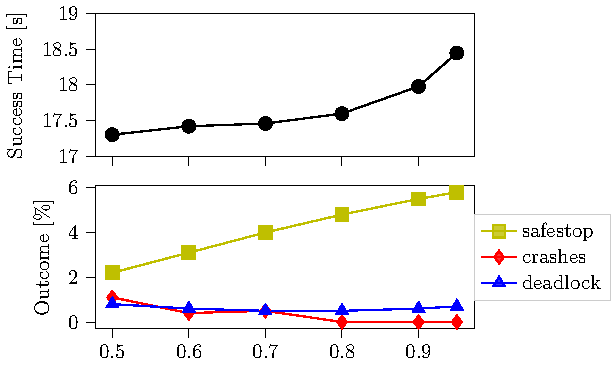
\includegraphics[width=0.99\columnwidth]{figures/figures-intention-t.pdf}
			% \include{tikz/results Intention threshold}
			% This file was created with tikzplotlib v0.10.1.
\begin{tikzpicture}

\definecolor{darkgray176}{RGB}{176,176,176}
\definecolor{goldenrod1911910}{RGB}{191,191,0}
\definecolor{green01270}{RGB}{0,127,0}
\definecolor{lightgray204}{RGB}{204,204,204}

\begin{groupplot}[group style={group size=1 by 2}]
\nextgroupplot[
height=3.5cm,
scaled x ticks=manual:{}{\pgfmathparse{#1}},
tick align=outside,
tick pos=left,
width=7cm,
x grid style={darkgray176},
xmin=-0.3, xmax=6.3,
xtick style={color=black},
xtick={0,1,2,3,4,5,6},
xticklabels={0.50,0.60,0.70,0.80,0.90,0.95,0.99},
xticklabels={},
y grid style={darkgray176},
ylabel={Success Time [s]},
ymin=14, ymax=20,
ytick style={color=black}
]
\addplot [semithick, black, mark=*, mark size=3, mark options={solid}]
table {%
0 14.9030054644809
1 15.7334844559585
2 16.1706398996236
3 16.541095890411
4 17.145
5 17.7761241291957
6 18.9131596526386
};

\nextgroupplot[
height=3.5cm,
legend cell align={left},
legend style={
  fill opacity=0.8,
  draw opacity=1,
  text opacity=1,
  at={(1,0.5)},
  anchor=west,
  draw=lightgray204
},
tick align=outside,
tick pos=left,
width=7cm,
x grid style={darkgray176},
xmin=-0.3, xmax=6.3,
xtick style={color=black},
xtick={0,1,2,3,4,5,6},
xtick={0,1,2,3,4,5,6},
xtick={0,1,2,3,4,5,6},
xtick={0,1,2,3,4,5,6},
xtick={0,1,2,3,4,5,6},
xticklabels={0.50,0.60,0.70,0.80,0.90,0.95,0.99},
xticklabels={0.50,0.60,0.70,0.80,0.90,0.95,0.99},
xticklabels={0.50,0.60,0.70,0.80,0.90,0.95,0.99},
xticklabels={0.50,0.60,0.70,0.80,0.90,0.95,0.99},
xticklabels={0.50,0.60,0.70,0.80,0.90,0.95,0.99},
y grid style={darkgray176},
ylabel={Outcome [\%]},
ymin=-1, ymax=100,
ytick style={color=black}
]
\addplot [semithick, green01270, mark=*, mark size=3, mark options={solid}]
table {%
0 73.2
1 77.2
2 79.7
3 80.3
4 80
5 78.95
6 74.85
};
\addlegendentry{goal}
\addplot [semithick, goldenrod1911910, mark=square*, mark size=3, mark options={solid}]
table {%
0 3.5
1 7.8
2 11.85
3 16.2
4 18.15
5 18.9
6 19.95
};
\addlegendentry{safestop}
\addplot [semithick, red, mark=diamond*, mark size=3, mark options={solid}]
table {%
0 23.25
1 14.95
2 8.25
3 3.3
4 1.35
5 0.95
6 0.85
};
\addlegendentry{collision}
\addplot [semithick, blue, mark=triangle*, mark size=3, mark options={solid}]
table {%
0 0.05
1 0.05
2 0.2
3 0.2
4 0.5
5 1.2
6 4.35
};
\addlegendentry{deadlock}
\end{groupplot}

% \draw ({$(current bounding box.south west)!0.5!(current bounding box.south east)$}|-{$(current bounding box.south west)!0.98!(current bounding box.north west)$}) node[
%   scale=0.5,
%   anchor=north,
%   text=black,
%   rotate=0.0
% ]{Intention threshold};
\end{tikzpicture}

			\vspace{-0.8cm}
			\caption{QMDP-IE success time for different $\zeta_\mathrm{threshold}$ values. Increasing $\zeta_\mathrm{threshold}$ lowers the collision rate while at the same time increasing the safe stop rate and the time it takes to reach a success state.}
	\label{fig:thesis_intent_threshold}
\end{figure}
In summary, while both QMDP and QMDP-IE rely on the Oracle DQN to predict Q-values, QMDP-IE reduces the complexity of decision-making by focusing on a single estimated intention state rather than a full belief state distribution reducing the computational complexity.

In the QID method, the intention state $\zeta^\mathrm{ID}_n$ is derived from the belief state $b$ using an approximator $D^\mathrm{ID}(b)$. The derived intention state $\zeta^\mathrm{ID}_n$ is obtained as the marginal distribution of intention from the set of particles $\{ x_m \}^M_{m=1}$: 
\begin{equation}
    D^\mathrm{ID}(b) = \zeta^\mathrm{ID}_n = [\zeta^\mathrm{ID}_\text{tw} \; \zeta^\mathrm{ID}_\text{yd}] = \sum_{m=1}^M w_{n[m]} [x(\zeta)]_{n[m]},
    \label{eq:ID_i}
\end{equation}
where each particle $x_m$ represents a possible state, and each particle has an associated weight $w_{n[m]}$, indicating its probability out of $M$ number of total particles.
The intention state used by the particle $[x(\zeta)]_{n[m]}$ is specified using a one-hot vector, which represents the intention state in a binary format where one element is '$1$' (indicating the active intention) and the others are '$0$'. The intention state for "take-way" is then $\zeta^\mathrm{ID}_\text{tw} \in [0,1]$ and consequently, "yield" becomes  $\zeta^\mathrm{ID}_\text{yd} = 1 - \zeta^\mathrm{ID}_\text{tw}$.
This process allows the QID method to derive a clear and actionable intention state from a distribution of possible states.

Both QMDP-IE and QID were evaluated on the intersection scenario introduced in Section~\ref{ch:simulation_env}, specifically designed to include at least one car on the intersecting lane with the same time to intersection as the ego vehicle. This scenario increases the likelihood of a collision if the intentions of the other vehicles are not accurately considered, thereby encouraging more safe stops.

\subsection{Results within the training set}

\begin{table}
	\caption{Result summary for scenarios within the training set}
	\label{tab:belief_results_summary}
	\begin{tabularx}{\columnwidth}{@{}l*{10}{c}c@{}}
	\toprule
	Experiments     & Goal reached & Safe stop & Collision & Deadlock & Success time \\ 
			 & $\%$ & $\%$ & $\%$ & $\%$ & s & \\ 
	\midrule
	Oracle DQN    & $84.50$ & $14.45$ & $1.05$ & $0.00$ & $15.49$\\ % $1\unit{\day}7\unit{\hour}$ \\ 
	% Noisy DQN & $84.25$ & $14.10$ & $1.65$ & $0.00$ & $15.48$ \\ 
	\textbf{QMDP-IE}   & $\textbf{80.00}$ & $\textbf{18.15}$ & $\textbf{1.35}$ & $\textbf{0.50}$ & $\textbf{17.14}$ \\ 
	% QMDP-IE   & $80.30$ & $16.20$ & $3.30$ & $0.20$ & $16.54$ & N/A \\ 
	QMDP      & $71.95$ & $15.05$ & $5.70$ & $7.30$ & $20.56$ \\ 
	% \arrayrulecolor{red}\hline
	% \arrayrulecolor{black}
	\textbf{QID}       & $\textbf{85.60}$ & $\textbf{10.40}$ & $\textbf{3.70}$ & $\textbf{0.30}$ & $\textbf{16.64}$ \\ %$\textbf{5\unit{\day}5\unit{\hour}}$ \\ 
	QPF       & $63.50$ & $21.80$ & $12.15$ & $2.55$ & $16.61$ \\ % $5\unit{\day}4\unit{\hour}$\\ 
	
	\bottomrule
	\end{tabularx}
\end{table}

This section presents the experimental results, starting with a comparison of the results of QMDP-IE and QID. QMDP is used as a baseline algorithm for QMDP-IE, while QPF, an algorithm trained on the whole belief state $b$ is used as the baseline for QID. Unlike QMDP-IE, the QID algorithm does not require access to the true intent during training.

As shown in Table~\ref{tab:belief_results_summary}, both QMDP-IE and QID beat their respective baseline algorithm in both higher goal reached and lowest collision percentage. QMDP-IE collision rate \SI{1.35}{\percent} was very close to the oracle DQN \SI{1.05}{\percent} making it as good as knowing the intention in these test cases.  
QID experienced more collisions than QMDP-IE but fewer than QMDP. This indicates that while training on ground truth is preferable, QID is a suitable alternative when ground truth data is not available.



\subsection{Results for scenarios outside the training set}
To investigate how the algorithms perform when exposed to behaviors they are not trained for, a scenario is introduced where a car is allowed to overtake another car in front, thereby violating the assumption of the \gls{idm}.
In the previous experimental scenario, the order of the other cars was structured such that if one car yielded, all following cars would stop behind it. This makes it possible to collide with a car that started behind a yielding car, but it also creates larger gap in between cars, that was not possible before. 

In this overtake scenario, both QID and QPF exhibit relatively low collision rates at \SI{2.53}{\percent} and \SI{3.7}{\percent} respectively. %, which are lower compared to the collision rates observed in the trained scenarios detailed in \ref{tab:belief_results_summary}. 
QMDP-IE and QMDP show slightly higher collision rates of \SI{4.6}{\percent} and \SI{5.95}{\percent} respectively, which is higher than QID and QPF and slightly higher than their own performance in the trained scenarios, detailed in Table~\ref{tab:belief_results_summary}. 
Because QMDP-IE uses the network from the Oracle DQN, it performs well when the intention is within the training set, while QID and QPF was trained on the uncertainty making the policy more cautious in zone 3 which lead to an opening in zone 2 leading to the goal. 
This suggests that QID is slightly better at taking passive actions in zone 3, which can change the intention distribution and reduce the uncertainty for the next state. This makes QID more effective at handling scenarios outside the training set than QMDP-IE.
% QMDP also has the highest safe stop and deadlock rate at \SI{10.2}{\percent} and \SI{4.15}{\percent}, making it the most passive policy. 

Overall, QID proves to be better than QMDP-IE in scenarios outside of the training set, offering more robustness to untrained behaviors. Meanwhile, QMDP-IE provides a structured approach with moderate collision rates and higher computational efficiency, performing well when the intentions are within the training set.

\begin{table}
	\caption{Results with an overtake agent}
	\label{tab:theis_results_overtake}
	\begin{tabularx}{\columnwidth}{@{}l*{10}{c}c@{}}
	\toprule
	Experiments & Goal reached & Safe stop & Collision & Deadlock & Success time \\ 
			 & $\%$ & $\%$ & $\%$ & $\%$ & s \\ 
	\midrule
	Oracle DQN & $89.80$ & $0.15$ & $10.05$ & $0.00$ & $16.01$ \\ 
	\textbf{QMDP-IE} & $\textbf{94.55}$ & $\textbf{0.20}$ & $\textbf{4.60}$ & $\textbf{0.65}$ & $\textbf{16.62}$ \\ 
	QMDP & $79.70$ & $10.20$ & $5.95$ & $4.15$ & $19.84$ \\ 
	\textbf{QID} & $\textbf{96.89}$ & $\textbf{0.11}$ & $\textbf{2.53}$ & $\textbf{0.47}$ & $\textbf{16.38}$ \\ 
	QPF & $96.15$ & $0.10$ & $3.70$ & $0.05$ & $17.62$ \\ 
	\bottomrule
	\end{tabularx}
	\end{table}
% \begin{figure}[!h]
% 	\centering
% 			% \includegraphics[width=0.99\columnwidth]{figures/results Scenarios 1-5 Take way Cars wo intent.png}
% 			% This file was created with tikzplotlib v0.10.1.
\begin{tikzpicture}

\definecolor{darkgray176}{RGB}{176,176,176}
\definecolor{goldenrod1911910}{RGB}{191,191,0}
\definecolor{green01270}{RGB}{0,127,0}
\definecolor{lightgray204}{RGB}{204,204,204}

\begin{groupplot}[group style={group size=1 by 2}]
\nextgroupplot[
height=3.5cm,
scaled x ticks=manual:{}{\pgfmathparse{#1}},
tick align=outside,
tick pos=left,
width=7cm,
x grid style={darkgray176},
xmin=-0.2, xmax=4.2,
xtick style={color=black},
ytick={13,15,17,19,21},
xtick={0,1,2,3,4},
xticklabels={1 car,2 cars,3 cars,4 cars,5 cars},
xticklabels={},
y grid style={darkgray176},
ylabel={Success Time [s]},
ymin=13, ymax=21,
ytick style={color=black}
]
\addplot [semithick, black, mark=*, mark size=3, mark options={solid}]
table {%
0 13.5619959677419
1 16.9007190265487
2 20.5162469536962
3 20.4080622347949
4 19.7671118530885
};

\nextgroupplot[
height=3.5cm,
legend cell align={left},
legend style={
  fill opacity=0.8,
  draw opacity=1,
  text opacity=1,
  at={(1,0.5)},
  anchor=west,
  draw=lightgray204
},
tick align=outside,
tick pos=left,
width=7cm,
x grid style={darkgray176},
xmin=-0.2, xmax=4.2,
xtick style={color=black},
xtick={0,1,2,3,4},
xtick={0,1,2,3,4},
xtick={0,1,2,3,4},
xtick={0,1,2,3,4},
xtick={0,1,2,3,4},
xticklabels={1 car,2 cars,3 cars,4 cars,5 cars},
xticklabels={1 car,2 cars,3 cars,4 cars,5 cars},
xticklabels={1 car,2 cars,3 cars,4 cars,5 cars},
xticklabels={1 car,2 cars,3 cars,4 cars,5 cars},
xticklabels={1 car,2 cars,3 cars,4 cars,5 cars},
y grid style={darkgray176},
ylabel={Outcome [\%]},
ymin=-1, ymax=100,
ytick style={color=black}
]
\addplot [semithick, green01270, mark=*, mark size=3, mark options={solid}]
table {%
0 99.2
1 90.4
2 61.55
3 35.35
4 29.95
};
\addlegendentry{goal}
\addplot [semithick, goldenrod1911910, mark=square*, mark size=3, mark options={solid}]
table {%
0 0
1 0.75
2 21.6
3 49.5
4 53.25
};
\addlegendentry{safestop}
\addplot [semithick, red, mark=diamond*, mark size=3, mark options={solid}]
table {%
0 0.8
1 8.85
2 16.85
3 15.15
4 16.8
};
\addlegendentry{collision}
\addplot [semithick, blue, mark=triangle*, mark size=3, mark options={solid}]
table {%
0 0
1 0
2 0
3 0
4 0
};
\addlegendentry{deadlock}
\end{groupplot}

% \draw ({$(current bounding box.south west)!0.5!(current bounding box.south east)$}|-{$(current bounding box.south west)!0.98!(current bounding box.north west)$}) node[
%   scale=0.5,
%   anchor=north,
%   text=black,
%   rotate=0.0
% ]{Scenarios 1-5 Take way Cars wo intent};
\end{tikzpicture}

% 			\vspace{-0.8cm}
% 			\caption{Performance results for DQN without intention state $\zeta$, showing success time and outcome percentage for scenarios with increasing numbers of other cars.}
% 	\label{fig:number_cars}
% \end{figure}


% \begin{figure}[h]
% 	\centering
% 			% 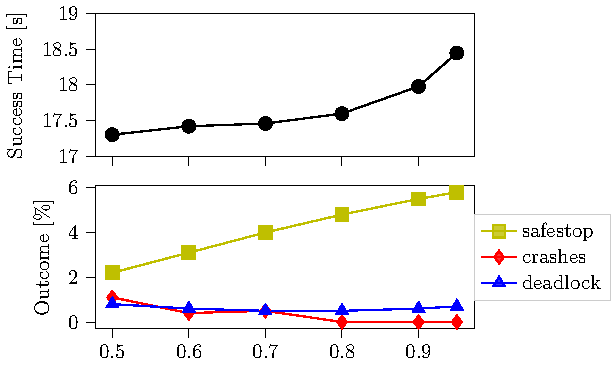
\includegraphics[width=0.99\columnwidth]{figures/figures-intention-t.pdf}
% 			% \include{tikz/results Intention threshold}
% 			% This file was created with tikzplotlib v0.10.1.
\begin{tikzpicture}

\definecolor{darkgray176}{RGB}{176,176,176}
\definecolor{goldenrod1911910}{RGB}{191,191,0}
\definecolor{green01270}{RGB}{0,127,0}
\definecolor{lightgray204}{RGB}{204,204,204}

\begin{groupplot}[group style={group size=1 by 2}]
\nextgroupplot[
height=3.5cm,
scaled x ticks=manual:{}{\pgfmathparse{#1}},
tick align=outside,
tick pos=left,
width=7cm,
x grid style={darkgray176},
xmin=-0.3, xmax=6.3,
xtick style={color=black},
xtick={0,1,2,3,4,5,6},
xticklabels={0.50,0.60,0.70,0.80,0.90,0.95,0.99},
xticklabels={},
y grid style={darkgray176},
ylabel={Success Time [s]},
ymin=14, ymax=20,
ytick style={color=black}
]
\addplot [semithick, black, mark=*, mark size=3, mark options={solid}]
table {%
0 14.9030054644809
1 15.7334844559585
2 16.1706398996236
3 16.541095890411
4 17.145
5 17.7761241291957
6 18.9131596526386
};

\nextgroupplot[
height=3.5cm,
legend cell align={left},
legend style={
  fill opacity=0.8,
  draw opacity=1,
  text opacity=1,
  at={(1,0.5)},
  anchor=west,
  draw=lightgray204
},
tick align=outside,
tick pos=left,
width=7cm,
x grid style={darkgray176},
xmin=-0.3, xmax=6.3,
xtick style={color=black},
xtick={0,1,2,3,4,5,6},
xtick={0,1,2,3,4,5,6},
xtick={0,1,2,3,4,5,6},
xtick={0,1,2,3,4,5,6},
xtick={0,1,2,3,4,5,6},
xticklabels={0.50,0.60,0.70,0.80,0.90,0.95,0.99},
xticklabels={0.50,0.60,0.70,0.80,0.90,0.95,0.99},
xticklabels={0.50,0.60,0.70,0.80,0.90,0.95,0.99},
xticklabels={0.50,0.60,0.70,0.80,0.90,0.95,0.99},
xticklabels={0.50,0.60,0.70,0.80,0.90,0.95,0.99},
y grid style={darkgray176},
ylabel={Outcome [\%]},
ymin=-1, ymax=100,
ytick style={color=black}
]
\addplot [semithick, green01270, mark=*, mark size=3, mark options={solid}]
table {%
0 73.2
1 77.2
2 79.7
3 80.3
4 80
5 78.95
6 74.85
};
\addlegendentry{goal}
\addplot [semithick, goldenrod1911910, mark=square*, mark size=3, mark options={solid}]
table {%
0 3.5
1 7.8
2 11.85
3 16.2
4 18.15
5 18.9
6 19.95
};
\addlegendentry{safestop}
\addplot [semithick, red, mark=diamond*, mark size=3, mark options={solid}]
table {%
0 23.25
1 14.95
2 8.25
3 3.3
4 1.35
5 0.95
6 0.85
};
\addlegendentry{collision}
\addplot [semithick, blue, mark=triangle*, mark size=3, mark options={solid}]
table {%
0 0.05
1 0.05
2 0.2
3 0.2
4 0.5
5 1.2
6 4.35
};
\addlegendentry{deadlock}
\end{groupplot}

% \draw ({$(current bounding box.south west)!0.5!(current bounding box.south east)$}|-{$(current bounding box.south west)!0.98!(current bounding box.north west)$}) node[
%   scale=0.5,
%   anchor=north,
%   text=black,
%   rotate=0.0
% ]{Intention threshold};
\end{tikzpicture}

% 			\vspace{-0.8cm}
% 			\caption{QMDP-IE performance (aggressiveness) for different $\zeta_\text{threshold}$ values. Increasing $\zeta_\text{threshold}$ lowers the collision rate while at the same time increasing the safe stop rate and the time it takes to reach a success state.}
% 	\label{fig:intent_threshold}
% \end{figure}

